\chapter{Research Plan}
\label{Chapter Research Design}
The analysis of BP algorithm for stereo matching is planned in two stages.

 \begin{enumerate}
   \item stage1: MRF formulation on stereo image
   \item Stage2: Applying  BP to minimize energy functions
The advantage of using Markov random field is that recovering the disparity map not only considering each individual pixel but also by considering neighboring pixel to find best match.
 \end{enumerate}


\begin{figure}
  % Requires \usepackage{graphicx}
  \includegraphics{rp1.eps}
  \caption{Research design } \label{rp}
\end{figure}





\section{MRF formulation on stereo image:}

MRF are undirected graphical model consist of nodes and links which encodes the spatial dependencies.
MRF is modelled on $3 \times3$ stereo image.
The diagram below shows about  MRF on $3\times3$ image.
\\The  blue nodes are observed variables which represents pixel intensity values where as pink nodes are hidden variables which represents disparity values are trying to find. The hidden values are referred as  labels.
The link between these node represents a dependency which is known as markov assumption.
\\A markov  assumption is that a node's state depends only on its immediate   neighbors .This assumption is used to  solve for the hidden  variables in a efficient manner.

The  stereo problem can formulate in terms of MRF as energy functions. The energy functions basically sum up all the cost at each link for a given image and label. The aim is to find label that produces lowest energy. The energy functions contains two functions, datacost function and smoothnesscost function.
\\The datacost function finds the cost of assigning label value ie. Disparity value to data ie. pixel intensity values. The function used for this is absolute difference function.
\\The smoothness function enforces smooth labeling across adjacent hidden nodes.

The  potts  model is a binary penalising function with a single tunable  variable. This value controls the smoothness of label.

\pagebreak
\begin{figure}[h]
\begin{center}
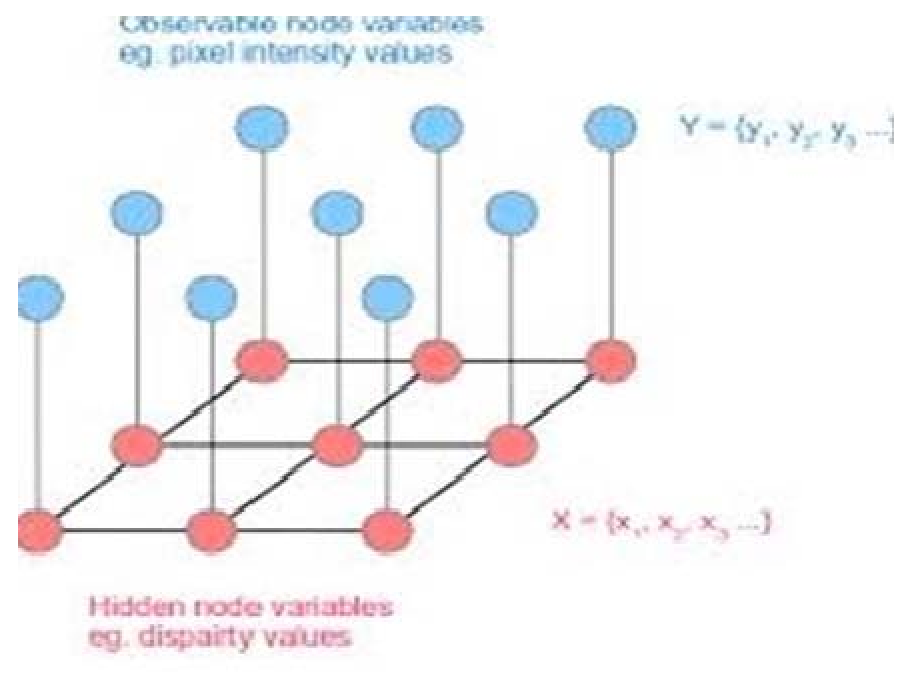
\includegraphics[width=3in]{mrf.eps}
\caption{MRF on 3x3 Image \cite{r11}} \label{mrf}
\end{center}
\end{figure}



\section{ Applying  BP to minimize energy functions:}

BP algorithm is one of the algorithm  used to find an approximate solution for an MRF.
\ BP is message passing algorithm , A node passes a message to an adjacent node only when it is received all incoming messages, excluding the message from the destination node itself.
Below diagram shows message passed from $x_{1}$ to$ x_{2}$

\pagebreak
\begin{figure}[h]
\begin{center}
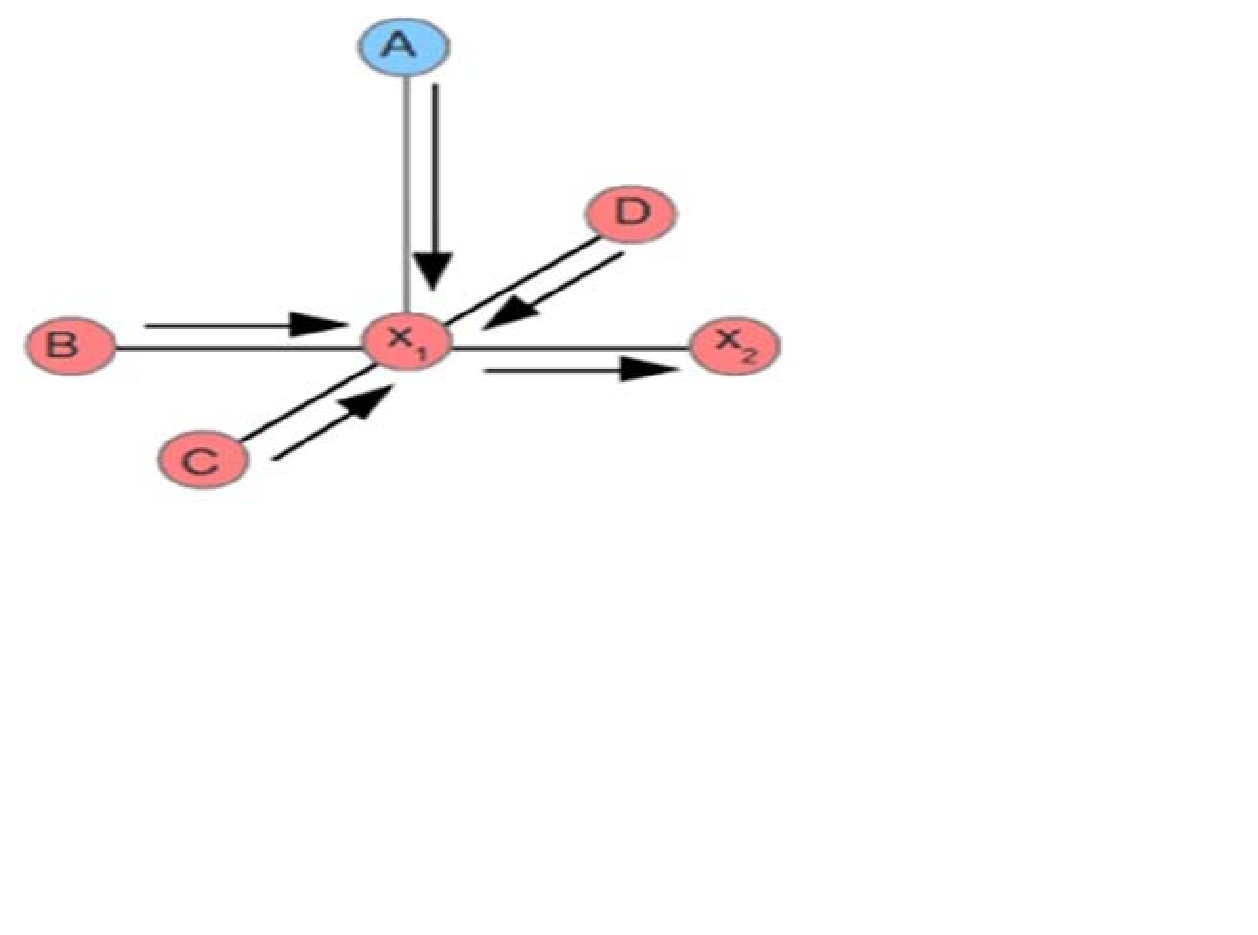
\includegraphics[width=3in]{bp.eps}
\caption{Message Passage in BP  \cite{r11}} \label{bp}
\end{center}
\end{figure}



To  implement Belief Propagation two decisions should be made
\pagebreak
\begin{figure}[h]
\begin{center}
\includegraphics[width=7in]{msgsc.eps}
\caption{Message schedule in BP } \label{msgsc}
\end{center}
\end{figure}



\begin{enumerate}
  \item First one is max-product algorithm is used  which finds the MAP estimate of the whole MRF
  \item The second choice is message update schedule determines when message send to the node will be used by that node to compute messages for the node's neighbors.
\end{enumerate}
 An message schedule is to propagate messages in one direction and update each node immediately.
For instance first node is in a row ,i would send message to the node at its right,i+1.Node i+1 would then use this message immediately along with the previously received from above and below to compute the message to the node i+2.
\\ Once this has been completed for every row,the same procedure occurs in the up,down and left directions. This schedule would only require one iterations for this information to propagated.
\\This feature of the $"up-down-right-left"$ message passing schedule causes the belief propagation algorithm to converge very quickly.
\\The diagram  below describes about Message schedule in BP.\\



The above mentioned plan is for this year\\
\subsection{The problem statement:}
By using different message passing schemes in belief propagation for stereo matching  can reduce computational time of algorithm.The execution time of belief propagation reduces after certain stability or convergence criteria met,but termination of algorithm is depend on  application of data.
\subsection{Expected Results:}
Development of a new or modify Belief Propagation optimization method by using different message passing scheme for stereo matching applications or cases of 3D objects.\\ And  Comparative analysis of new method with existing method.\\
 MATLAB is used to simulate functions in the proposed  research work.



